%!TEX root = ../thesis.tex
%*******************************************************************************
%****************************** Fourth Chapter **********************************
%*******************************************************************************
\chapter{A Web Interactive Tool for Exploring High-Dimensional Data}
\label{chapter4}

\graphicspath{{Chapter4/figs/}}

%% Cites required
One of the main focus of the state of the art proposals in Interactive ML is to provide user with the ability for model space exploration looking to produce a good representation of embeddings and clusters. The discussion about what is a good representation, being the general problem in unsupervised learning, continues open. In addition, researchers also focus on deriving the most relevant interaction elements for supporting the data exploration. These proposals can be complemented with components for data exploration and navigation, being this a mandatory stage in any data analytics study, and model results understanding in terms of attributes in the original space.  In this work, a web interactive tool more suitable for domain-experts users with cluster-oriented tasks in high-dimensional data rather than just interaction with DR and Clustering models is presented. Design decisions about components or functionalities provided by the tool are explained in the subsequent sections. 

In addition, the decision behind implementing the tool in a web-based environment with local ML computation using only JavaScript libraries for shareability, interactivity and on-device computation is inspired by \cite{Smilkov2019TensorFlow.js:Beyond}. These properties are important for domain-expert users because enable them to perform ML-based EDA without requiring complex infrastructure and easily share their work with colleagues and community in general. By the other hand, local computation also has the advantage of privacy preserving, because despite the tool is available on internet, the data remains in the browser. 

\section{Load Dataset}
\label{load-dataset-section}

In many cases, domain-expert users store data in local semi-structured files, principally when the size does not demand to invest resources to maintain TI infrastructures increasing the complexity of the project.
The tool supports loading datasets from a local path in CSV format and file size constraint depends on browser capabilities. In addition, as sown in Figure \ref{fig:load-dataset-component}, some low size datasets for trainees are available: (1) the Fisher's Iris \cite{FisherIris}, the Zoo dataset \cite{*}, the Breast Cancer dataset \cite{*} and the Heart Diseases dataset \cite{*}.

\begin{figure}[ht]
 \centering
 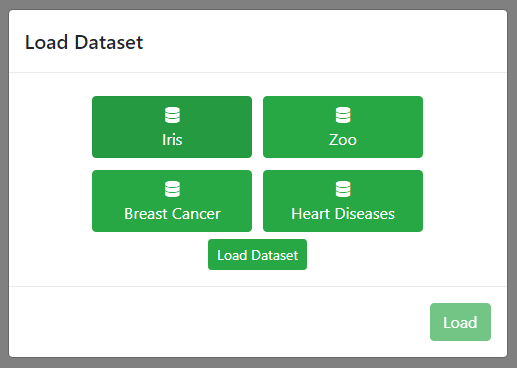
\includegraphics[width=0.5\textwidth]{load_dataset.png}
 \caption{Load Dataset component.}
 \label{fig:load-dataset-component}
\end{figure}

\section{Attribute Selection}
\label{attribute-selection-section}

Attribute selection is an important stage in any ML process. After the user load a dataset, all attributes are listed including an icon representing its type and a checkbox for attribute selection. Currently, the tool is able to identify three types of attributes: numerical, boolean and categorical or strings. Boolean type is automatically identified when the attribute has only two values: 0 and 1. By default, all numerical and boolean attributes are selected meaning that these will be used for training the models. The reason behind this decision is related to the constraint of the models available in the tool of working only with numerical data. Nevertheless, categorical attributes are available for color encoding representing classes or clusters. The user can select the attribute for color encoding in the upper-right combobox, the tool automatically selects a categorical attribute with low cardinality. Figure \ref{fig:attribute-selection-component} shows the Attribute Selection component for the FIFA dataset.

\begin{figure}[ht]
 \centering
 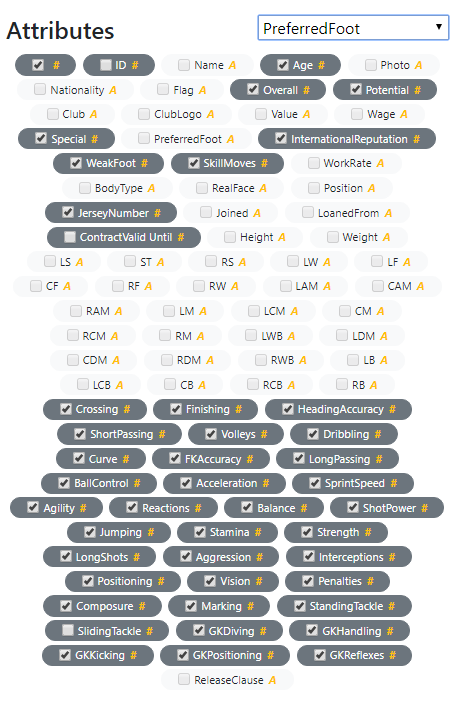
\includegraphics[width=0.5\textwidth]{attribute-selection.png}
 \caption{Attribute Selection component.}
 \label{fig:attribute-selection-component}
\end{figure}

\section{Data Exploration and Navigation (Navio)}
\label{navio-section}

The intention of using ML for exploring high-dimensional data does not imply that user should forget about descriptive techniques enabled also for gaining data understating. Distribution summarization, correlation analysis and outliers identification, among others, are generalized user tasks that always must be covered in any analytic process. Navio \cite{Guerra-Gomez2018Navio:Datasets} is an interactive web-based tool designed for achieving these kind of tasks but also for data navigation implementing three interactions: sorting, filtering a range and filtering by value. Because this tool is available as a JavaScript widget, the incorporation as a component complementary to attribute selection-level interactions looking for a more informed ML models usage is highly valuable for domain-expert users. Figure \ref{fig:navio-component} shows the Navio component for the FIFA dataset.  

\begin{figure}[ht]
 \centering
 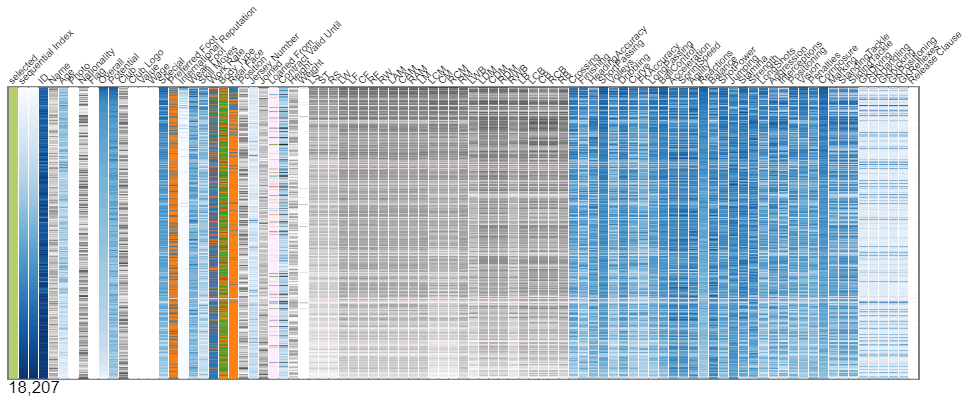
\includegraphics[width=0.9\textwidth]{navio.png}
 \caption{Data Exploration and Navigation (Navio) component.}
 \label{fig:navio-component}
\end{figure}

\section{Model Space Exploration}
\label{model-space-exploration-section}

The user is enabled to train in the browser two kind of models for supporting the cluster-oriented EDA: t-SNE \cite{VanDerMaaten2008} and K-Means \cite{Lloyd1982LeastPCM}. 

%In order to provide a mechanism to carry out cluster-oriented task sequences, as defined in \cite{*}, user can select a categorical attribute for color encoding, in the case of labeled data, but in general we provide an additional functionality to train a K-Means clustering model and use its results for color encoding.

%For both algorithms, t-SNE and K-Means, user is able to modify the model hyper-parameters and visualize how embedding is affected in an iterative way. 

\section{Results Understanding}
\label{results-understanding-section}

The last component is based on proposals for local interpretability like LIME \cite{Ribeiro2016} and extensions

%Because Inter2DR is a tool for domain-expert users, we decide to include two complementary groups of idioms to validate the embedding and clustering models by observation of independent attribute distributions and instance details in a table. These components present coordinate highlighting, enabling user to quickly compare instances in the embedded space with their attribute values in the original space and vice versa.

\section{Reproducing Experiments}
\label{results-understanding-section}

Finally, in any stage of the experimentation user is able to locally save and load a configuration file. This file contains a list of the attributes, their type and which of these were used to train the models and encode the color. Currently, the configuration file only stores the hyper-parameters and results of the last trained models for the t-SNE and K-Means algorithms. Another limitation of this component is related to storing the Navio state, meaning that the interaction sequence for sorting or filtering carried out during the previous experimentation cannot be reproduced. In other words, user is able to observe the results of a previous experiment and re-train the models using the same hyper-parameters for achieving comparable results only if the dataset was not filtered. 